\documentclass[sigplan]{acmart}\settopmatter{printfolios=true,printccs=false,printacmref=false}

\acmConference[NCSU, FALL 2018]{CSC791 - Foundation of Software Science}{December 7, 2018}{Raleigh, NC, USA}
\acmYear{2018}
\acmISBN{} % \acmISBN{978-x-xxxx-xxxx-x/YY/MM}
\acmDOI{} % \acmDOI{10.1145/nnnnnnn.nnnnnnn}
\startPage{1}
%\renewcommand{\baselinestretch}{1.00} 


\setcopyright{none}


\usepackage{booktabs}   %% For formal tables:
                        %% http://ctan.org/pkg/booktabs
\usepackage{subcaption} %% For complex figures with subfigures/subcaptions
                        %% http://ctan.org/pkg/subcaption


\begin{document}

%% Title information
\title[Comparison of Tree based Learners in Incremental Dataset of Software Defect Predictions - A Case Study]{Comparison of Tree based Learners in Incremental Dataset of Software Defect Predictions - A Case Study}         
\subtitle{}                    


\author{Md Rayhanur Rahman}
\authornote{unity id: 200255928}          %% \authornote is optional;
                                        %% can be repeated if necessary
\orcid{nnnn-nnnn-nnnn-nnnn}             %% \orcid is optional
\affiliation{
  \position{Ph.D. Student}
  \department{Dept. of CSC}              %% \department is recommended
  \institution{NC State University}            %% \institution is required
  \city{Raleigh}
  \state{NC}
  \country{USA}                   %% \country is recommended
}
\email{mrahman@ncsu.edu}          %% \email is recommended



\begin{abstract}
In various research fields, data miners are being applied in an intense manner such as in domains of computing, space, business intelligence etc. In software engineering domain, it is also being used extensively. One of the key area where it is being applied is defect prediction. Defect prediction models helps software developers to control the quality issues of the software projects. There are a diversified range of data miners utilized to predict defects from the software metrics such as simple regressors and classifiers as well as complex multi objective models. These days, source codes of the software can be obtained from the github and other repositories easily and code metrics can be computed on the fly. This indicates that datasets for defect prediction can grow to a large volume incrementally over time. In such scenario, scalability challange will appear as the data become larger and larger. In this research, we will try to compare the offline tree based classifiers and online VFDT classifier to observe the case of classifiying defects from large datasets. From our observation, we found out that, online classifier behaves more stable and produces similar results without paying the penalty of time.  
\end{abstract}

\keywords{Defect Prediction, Decision Tree, Random Forest, VFDT, FFT, Online Analysis }

\maketitle

\section{Introduction}
These days, software automation has engulfed all the spheres of our life. Millions of software companies automates new business logics along with replacing legacy systems with its modern descendant. Consequently, software development is an ongoing process that never stops and hence, there will be always defects in the software sources that needs to be fixed in constant manner. Fixing these defects is one of the key concern in software quality assurance activities and dedicated human resources spend a significant time in resolving these issues - if unfixed, culminates in loss of money, time, consumer satisfaction and in mission critical cases, casualties.  

Finding and fixing software defects was a manual task decades ago. But these days, data miners are there to help the developers find these defects. These data miners work on the defect prediction models that mainly contains software code quality metrics such as line of code, cyclometric complexity etc. Based on these data, those data miners predicts whether a particular software module would contain defects or not.  

...To perform defect prediction studies, researchers have explored the use of various classification techniques to train defect prediction models. For example, in early studies, researchers used simple techniques like logistic regression and linear regression to train defect prediction models. In more recent work, researchers have used more advanced techniques like adaptive regressions, ensemble learning etc. Several context sensitive analysis based defect predictors are explored as well.  

...Despite the fact that, there have been numerous advanced miners deployed in defect prediction; classification techniques to build defect prediction models have focused on the performance. However, as the volume of software source codes increases in daily basis, so does the size of defect prediction examples from which the classifiers will predict the defects. Hence, in case of traditional learners, memory and sample size will be a dominant obstacle if those are fed with incrementally large amount of data from time to time. Being trained with small number of data also suffers from overfitting. Meanwhile, currently there are many online data-miners are available which are sample size agnostic. Thus exploring the comparison of traditional learners and online data miners have become a priority.  

In this paper, we have put three offline classifiers named CART decision tree based classifier, Fast Frugal Tree (FFT), Random forest against online classifier named VFDT. We will look into three research questions in particular:
\begin{itemize}
	\item \textbf{RQ1: } How these four classifiers performs in large defect prediction datasets that will increment over time
	\item \textbf{RQ2: } How hyper-parameters changes as the data size changes
	\item \textbf{RQ3: } How much computation resources would be used by these four learners 
\end{itemize}

We have used four defect prediction datasets obtained from (...). These datasets contains around $40,000$ examples on an average. From our observation we found out that, VFDT performs better and more stable manner than the other three as the data size increases. Moreover, the performance differential becomes more prominent among those learners considering datasize increase and finding tuning parameters.  

Rest of the paper is organized as follows. In the section II, we will discuss existing literature study on this aspect. In section III, we will discuss baseline criteria upon which we will evaluate our comparison of the learners, In section IV, we will discuss the experiment setup and result analysis. Finally, it will be followed by discussion and future work scope in the section V. 

\section{Related Work}
bla bla bla

\section{Background and Motivation}
...
\subsection{Baseline Criteria for Data Miners} These days, numerous data miners are being deployed in SE domain. There are also a diversified variation in how those miners tweaked and tuned to fit a particular model. That leaves us with virtually unlimited choice to pick a certain data miner or optimizer to apply in a new problem. However, according to the no free lunch theory, these is no single miner which would suit best in every possible models. So, we need to apply commissioning to filter through the possible choices of data miners or optimizers. In that regard, baseline criteria is truly useful. Baseline criteria refers to the important factors, majority of which should be achieved by a learner. It provides key insight to us regarding how effective and efficient the data miners would perform in the real world. Here follows some of the key baseline crietria along with their short description. 
\subsubsection{Simple and Reasonable}

Learners should be simple in a sense that it is easily explicable to the end users. It should also be easy to understand the underlying models, how it works and how to work on to build on further. There are several learners that not very easy to describe such as Naive Bayes classifiers and neural networks. On the other hands, decision tree based models are simple enough to understand and explain to others. However, learners have to be reasonable as well. It should perform well in terms of accuracy and performance. Otherwise being a simple learning producing non-reasonable results does not help the case of data mining activities. 

\subsubsection{Stable and Robust}
Data miners work on examples to build the model and on the basis of that model, make the predictions. Datasets containing loads of examples poses a significant challenge for the miners. Datasets comes with lots of unique cases as well context aware information. Some datasets are also imbalanced while the others might be incomplete. There is also a potential chance of a lot of anomalies hidden in the dataset.  All these factors contribute to the fact of being a data miner unstable. This means the learner would produce different type of decisions in case of diversified datasets which is extremely frustrating for business users. It also prevents further improvement of the data miners. Data miners also need to be robust throughout most of the cases of different sample size, splits and validation techniques.  

\subsubsection{Generic}
Data miners should be as generic as possible referring to the fact that they should provide a range of possible solution rather than a simple one point one. The benefit of it is to help the end users with a possible wide outlook of the scenario. But if the miners behave too specific or provides only one solution of a certain scenario, it would confuse the end users more. There is also a chance to miss other corner cases and ignore other possible, equally similar solutions which would turn out truly bad in real world scenario.  

\subsubsection{Replicable}
The learner should build model from the dataset and produce outputs fast enough. This ensures that the learner can be invoked iteratively in case of learning, understanding, rebuilding or tweaking. If it takse several hours to produce outputs for a small data, it would become impossible to work on that learner or tune a little bit. At the same time, the learner must also produce the same output every time if is fed the same input. If the outcome of a certain learner is not replicable, then it is impossible to understand, implement and improve the learner. 

\subsubsection{Goal Aware}
These days, all the real world problems do not focus on a single goal. Earlier, optimizers were used to maximize or minimize a value over a set of constraints but now a days, complex situations are there where there is no optimal solution. Hence, data miners being applied in those fields should be goal aware. This means, rather focusing on a single goal, the miner should produce output in such a manner so that the output should reflect overall realization of multiple goals. There might be conflicting goals and often, the correlation of the goals and datasets are quite complex. None the less, the miner should be able to handle such conflicts, complexity and tradeoff cases and produce results that provides a satisfaction of all the goals.  

\subsubsection{Anomaly Aware}
It is almost certain and usual that the datasets would contain a percentage of noisy and anomalous examples. Data miners should be able to detect and cancel out those. However, sometimes data miners confuses with the true example as anomalous examples and thus discards those or learn something misleading. A good data miner should be able to handle all these cases.

\subsubsection{Context Aware}
Despite the fact that a dataset should represents a generic scenario of a particular phenomenon, often this is the case that many context specific information are hidden in the datasets. So in the datasets, there might be a region of locality which is almost similar to other generic examples but might vary in one or two attributes and indicates different labels. Those regions are in fact, responsible for difference in decision making process. Thus, a good data miner should be able to find out those context specific local regions and learn the phenomenon protecting the generic learning model intact as well. This baseline is very critical in fields of health, e-commerce etc.

\subsubsection{Incremental}
Modern days, datasets tend to be large. They also get incremented periodically. So it is in vain if a data miner build models from a datasets and then can't reuse the already built model if it wants consider the newer example. So data miner should be able to extend the existing knowledge of model reading the newer examples. It should also be able to run over infinite stream of datasets as well as relearn in case of anomalies. 

\subsubsection{Shareable}
The datasets and the obtained knowledge by the learner should be shareable so that the obtained learning can be obtained in different contexts. However, while sharing the datasets, privacy should be a big concern. So miners should be able to hide the actual data and interpret the outcomes at the same time so that sensitive information of the datasets are protected. 

\subsubsection{Tunable}
There are a variety of parameters on every learners that can affect the accuracy, performance and stability of the learners. However, for a large datasets, if it is necessary to find the best set of tuned parameters for the miner, then it would take a hefty amount of time to do so. So a data miner should be able to tune itself so that it can be fit to a certain dataset or certain domain specific models to obtain better results. 

In addition, there are several other baselines that deserves mention:
\begin{itemize}
	\item Be applicable to mixed qualitative and quantitative data
	\item Have no parameters within the modelling process that require tuning.
	\item Be publicly available via a reference implementation and associated environment for execution
	\item Be computationally cheap in a reasonable sense
\end{itemize}

\subsubsection{Criteria for this Work}
All of the aforementioned criteria are more or less critical for any learner. However, set of baselines critical for a particular domain depends on many contexts as well. In some cases, computational performance might be the most critical. In other case, the accuracy might be the most critical one. In the context of this work, we will try to observe the performance of various tree based learners on incremental data. Hence, for our work, here are the list of critical baseline we will look more closely:
\begin{enumerate}
	\item \textbf{Usefulness: } The output of the miners should be at least better than some random guess. In this work, the miner would predict whether a given example contains bugs or not. The typical evaluation metrics such as precision and recall of the learners would be put into the focus. The examples will be fed into the miners in an incremental manner and we would observe how those evaluation measure changes over the new datasets that fed into the learners.
	\item \textbf{Stable: } Stability is quite important in case of prediction. If the output of the learners produces varying degree of outputs, then the decision making process would be frustrating. In the context of this work, we would look into the stability of the prediction of the learners in terms of incrementally updated set of examples and observe how these learners perform.
	\item \textbf{Cheap: } The computational resources being used by the learners is another important aspect. Learners might produce great results but if it comes using heavy computational resources such as cpu time and memory, then it might not become that useful in real world scenario. In this work, learners will learn from a range of small datasets to large one. So, we will try to gather information on how much cpu time and memory resources those learner will use to produce results.
	\item \textbf{Robust: } In case of incremental datasets, the learners need to accommodate all the newer examples. However, this might also confuse learners with different examples or noisy examples. So it needs to be seen how robustly the learner can handle all the examples that will be added in the larger datasets.
	\item \textbf{Streaming: } In case of very big datasets, the learners should be able to stream in the newer examples and fit those in the existing models. Otherwise, the learners need to completely relearn everything in case of the arrival of the newer data. In the context of this work, this is a very critical requirement.
	\item \textbf{Tuning: } Tuning of the parameters of the learners is another important baseline. In our case, we would feed the learners with increasingly bigger amount of example set and observe how the initial tuning performs for the rest of the data. We would also like to observe how the optimal set of tuned parameters changes when newer examples comes into the context.
\end{enumerate}

\subsection{Motivation}
These days, source codes are being committed to the source code repository periodically. The frequency of committing newer code base is ranged from hours and to days. In order to help developers with new potential defects while the new code base being committed, need to relearn the whole defect prediction model is necessary. As the new code is being pushed, software source code metrics which are being used be defect prediction models needs to be recomputed. Hence, the newer examples of software defects would come into play. So, assuming that newer version of source code being committed to the repository at least once in a day results into re-computation and relearning the whole things from the scratch. Traditional decision tree based learners such as Classification and Regression Tree, Random Forest, Fast frugal Trees all would need to relearn everything which is very cpu and memory extensive. If, high speed stream based learners would have been used in this scenario, then there would be no need to relearn everything from scratch as the streaming data miners automatically accommodates the newer examples with the existing models. That signifies the motivation of this work. We would like to observe how streaming learners perform against the offline learners in terms of feeding newer set of examples periodically. Hence, in this work, we would compare CART, RF and FFT against VFDT which is an online stream based decision tree learner and compare all these learners from the aspect of aforementioned baseline criteria.

\subsection{Classifiers}
In this work, we will observe the performance of four decision tree based classifiers. Here is a short description of each of these classifiers.

\subsubsection{Decision Tree}
Decision Tree learners uses decision tree based models as a predictive model to perform classification or regression over a set of examples. In our case, we will only use classification trees where the tree will be used to predict the class labels of a given set of examples. Each interior node refers to independent variables and edges refers to the value of that independent variable. Each leaf corresponds to the value of a target variable (or label or class) on the basis of all independent variables lying on the path from root to leaf. Each of these internal nodes are computed recursively from root. First, from the root, the best attribute is chosen on the basis of information gain from that attribute. After selecting the first best attribute, the root will have children based on the attribute value. Then in each of the child nodes, this process will go on recursively. The stopping criteria can be either a threshold of information gain or the depth of the tree. The leaves of the tree contains the probability of each labels associated with the choice of independent attributes from root to the leave. The advantage of decision tree is that it is simple, understandable and interpretable. It can handle both numerical and categorical data and it can be used to multiple classification and regression problem. However, decision trees would suffer from overfitting issue. Sometimes, the constructed decision model is very complicated as well. It also become unstable sometimes due to the variation in the training datasets. Moreover, finding the optimal decision tree for a particular model is not straightforward process. In the scope of this work, we will use the standard decision tree library from the python scikit-learn package. It uses an optimized version of CART (classification and regression Trees) which is a variant of C4.5 decision tree. 

\subsubsection{Random Forest}
Random Forest is an ensemble learning methods where multiple decision trees will be constructed from the training class and during testing, the class will be predicted that is the mode class predicted by all of the decision trees of that random forest. The intuition of random forest is to tackle the problem of overfitting suffered by the decision trees. In order to build the decision trees during the training time, example data of the training dataset will be randomly chosen along with replacement. During the computation of best splitting criteria, it would do that so from a randomly selected subset of the training example set. As a result, each tree tends to tackle the biasness and bagging along with random subset selection also ensures that individual trees have low correlation to each other leading to an ensemble that is both of low bias and low variance. In the scope of this work, we use the Random Forest library from scikit-learn package.

\subsubsection{Fast and Frugal Tree}
Fast and Frugal trees is a type of decision tree where a set of hierarchical rules is obtained from a training set. This tree has a depth of four usually and two branches in the each node. Each node represents a splitting attribute associated with a certain value or range. One of the branch denotes the subtree which will be used for further training if the condition is satisfied. The another branch is simply a leaf which denotes the cases if the condition is no satisfied. The leaf also contains the class information with associated probability. This type of tree is useful for quick interpretation of the decision models obtained from a training dataset. It is also useful for the dataset where number of key attributes is more or less, equal to the depth of the decision tree. In this work, we have implemented the Fast and Frugal tree from the scratch. We have used unsupervised discretization to select the best splitting attribute. 

\subsubsection{VFDT - Very Fast Decision Tree}
Classic decision tree learners like ID3, C4.5 and CART assume that all training examples can be stored simultaneously in main memory, and are thus
severely limited in the number of examples they can learn from. Disk-based decision tree learners like SLIQ [10] and SPRINT [17] assume the examples are stored on disk, an 
learn by repeatedly reading them in sequentially (effectively once per level in the tree). While this greatly increases the
size of usable training sets, it can become prohibitively expensive when learning complex trees (i.e., trees with many levels), and fails when datasets are too large to fit in the
available disk space

Our goal is to design a decision tree learner for extremely large (potentially infinite) datasets. This learner should require each example to be read at most once, and only a small
constant time to process it. This will make it possible to directly mine online data sources (i.e., without ever storing the examples), and to build potentially very complex trees with
acceptable computational cost. We achieve this by noting with Catlett [2] and others that, in order to find the best attribute to test at a given node, it may be sufficient to consider only a small subset of the training examples that pass 
through that node. Thus, given a stream of examples, the first ones will be used to choose the root test; once the root attribute is chosen, the succeeding examples will be passed
down to the corresponding leaves and used to choose the appropriate attributes there, and so on recursively.1 We solve the difficult problem of deciding exactly how many examples are necessary at each node by using a statistical result known as the Hoeffding bound (or additive Chernoff bound). Consider a real-valued random variable $r$ whose range is $R$ (e.g., for a probability the range is one, and for an information gain the range is log $c$, where $c$ is the number of classes). Suppose we have made $n$ independent observations of this variable, and computed their mean $\bar{r}$. The Hoeffding bound states that, with probability $1-\delta$, the true mean of the variable is at least $\bar{r}-\epsilon$ , where 
\begin{equation}
	\epsilon = \sqrt{\frac{R^2\ln(1/\delta)}{2n}}
\end{equation}

\begin{figure}
	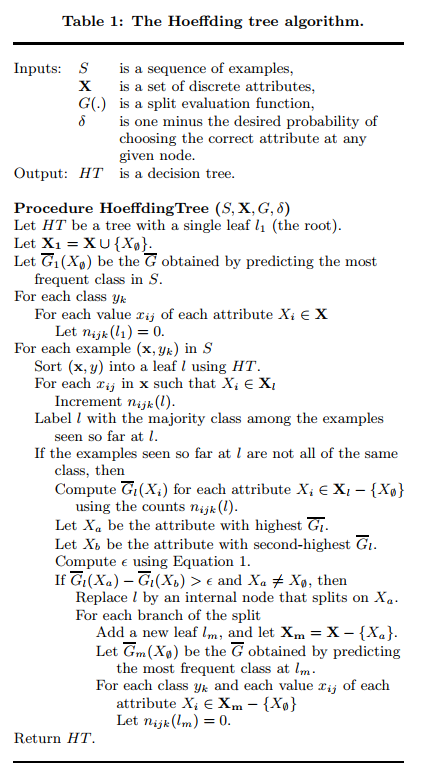
\includegraphics[width=\linewidth]{figs/vfdt.PNG}
	\caption{The VFDT Algorithm}
	\label{fig:vfdt}
\end{figure}

The Hoeffding bound has the very attractive property that it is independent of the probability distribution generating the observations. The price of this generality is that the bound is more conservative than distribution-dependent ones (i.e., it will take more observations to reach the same $\delta$ and $\epsilon$). Let $G(X_i)$ be the heuristic measure used to choose test attributes (e.g., the measure could be information gain as in C4.5, or the Gini index as in CART). Our goal is to ensure that, with high probability, the attribute chosen using $n$ examples (where $n$ is as small as possible) is the same that would be chosen using infinite examples. Assume $G$ is to be maximized, and let $X_a$ be the attribute with highest observed $\bar{G}$ after seeing $n$ examples, and $X_b$ be the second-best attribute. Let $\Delta \bar{G} = \bar{G}(Xa) - \bar{G}(Xb) \ge 0$ be the difference between their observed heuristic values. Then, given a desired $\delta$, the Hoeffding bound guarantees that $X_a$ is the correct choice with probability $1 - \delta$ if $n$ examples have been seen at this node and $\Delta \bar{G} > \epsilon^2$ In other words, if the observed $\Delta \bar{G} > \epsilon$ then the Hoeffding bound guarantees that the true $\Delta G \ge \Delta \bar{G} - \epsilon > 0$ with probability $1 - \delta$, and therefore that $X_a$ is indeed the best attribute with probability $1 - \delta$. This is valid as long as the $G$ value for a node can be viewed as an average of $G$ values for the examples at that node, as is the case for the measures typically used. Thus a node needs to accumulate examples from the stream until $\epsilon$ becomes smaller than $\Delta \bar{G}$. (Notice that $\epsilon$ is a monotonically decreasing function of $n$.) At this point the node can be split using the current best attribute, and succeeding examples will be passed to the new leaves. This leads to the Hoeffding tree algorithm, shown in pseudo-code in \ref{fig:vfdt}.


A key property of the Hoeffding tree algorithm is that it is possible to guarantee under realistic assumptions that the trees it produces are asymptotically arbitrarily close to the ones produced by a batch learner (i.e., a learner that uses all the examples to choose a test at each node). In other words, the incremental nature of the Hoeffding tree algorithm does not significantly affect the quality of the trees it produces. In this work, we have implemented vfdt by python completely from the scratch. 

\subsection{Tuning Method}
As CART, Random Forest and VFDT have several parameters that can pose impact in the classification performance, parameter tuning is necessary before deploying the learners for classifications tasks. We have used differential evolution method for finding the sub-optimal parameters for the classifiers. It finds the optimal solution for a problem by iteratively searching the canditate solution on the basis of a given fitness function. First it generates an initial population of candidate solutions and then generate subsequent set of candidate solutions by applying mutation and crossover methods. After that, all the possible solutions will be tested against a fitness function and best set of solutions will be kept. This process is done iteratively for several pass and final set of best solution will be considered. However, it must be kept in mind that this process does not guarantee that the theoretical optimal solution has been found. In this work, we have implemented this process from the scratch. 


\section{Experiemnt Design}
In this work, we will apply four data miners named CART, FFT, RF and VFDT on four software defect prediction datasets. These datasets will be fed to the miners incrementally. We would observe the performance of all four miners based on these datasets. The experiment setup is described below:

\subsection{Dataset}
Although, there are so many standard defect prediction datasets, we choose use datasets that came from different sequential committed version of the same source code. It will allow us to experiment with large set of examples and incremented examples over a period of time. Here is the descriptions of the datasets:

\begin{center}
	\begin{table}[h]
			\begin{tabular}{|c|c|c|}
			\hline 
			\textbf{Name} & \textbf{Examples} & \textbf{Attributes} \\ 
			\hline 
			abinit & 89303 & 29 \\ 
			\hline 
			lammps & 41130 & 40 \\ 
			\hline 
			libmesh & 24673 & 40 \\ 
			\hline 
			mdanalysis & 11694 & 37 \\ 
			\hline
		\end{tabular}   
	\caption{Dataset Description}
	\label{tab:dataset}
	\end{table}
\end{center}

After choosing the datasets, training and test example set needs to be generated. However, stratification and n-fold cross validation are not an option because those examples in the datasets are needed to be fed into the miners in incremental order (i.e. $5\%, 10\%, 15\%... $ of the data). This is why we randomly choose $80\%$ of the examples for each dataset and keep the rest of the data for testing set without breaking the sequence of the data. Thus, we have generated 10 different set of training and testing example pairs for each dataset. 

\subsection{Testbed Setup}
The work is performed in a traditional laptop PC. Here is the information of the execution environment.

\begin{center}
	\begin{table}[h]
		\begin{tabular}{|c|c|}
			\hline 
			OS & Ubuntu 18.04 \\ 
			\hline 
			CPU & Intel Core i7 8550U \\ 
			\hline 
			Memory & 16GB \\ 
			\hline 
			Disk & SSD 240GB \\ 
			\hline 
			Language & Python 3.6 \\ 
			\hline 
			Data Miner Library & Scikit-Learn 0.20 \\ 
			\hline  
		\end{tabular} 
	\caption{Testbed Information}
	\label{tab:testbed}
	\end{table}
\end{center}

\subsection{Parameter Tuning}
As CART, Random Forest and VFDT have several parameters that can pose impact in the classification performance, parameter tuning is necessary before deploying the learners for classifications tasks. Here is the last of parameters that are needed to be tuned for the classifiers.

\begin{enumerate}
	\item \textbf{Number of estimators: } This parameter is only applicable to random forest classifier. This is the number of trees that will be used for classification task in the random forest. 
	\item \textbf{Tree depth: } This parameter denotes the maximal depth of the decision tree.
	\item \textbf{Minimum sample leaves: } This denotes the minimum number of samples required to split an internal node.
	\item \textbf{Minimum number of examples to split: } This denotes the minimum number of samples required to be at a leaf node. A split point at any depth will only be considered if it leaves at least of this value in each of the left and right branches.
	\item \textbf{Ties: } When two or more attributes have very similar $G$s, potentially many examples will be required to decide between them with high confidence. This is presumably wasteful, because in this case it makes little difference which attribute is chosen. Thus VFDT can optionally decide that there is effectively a tie and split on the current best attribute if $\delta G < \epsilon < \tau$, where $\tau$ is a user-specified threshold.
	\item \textbf{Frequency of Computation of $G$: } The most significant part of the time cost per example is recomputing $G$. It is inefficient to recompute G for every new example, because it is unlikely that the decision to split will be made at that specific point. Thus VFDT allows the user to specify a minimum number of new examples nmin that must be accumulated at a leaf before $G$ is recomputed. This effectively reduces the global time spent on $G$ computations by a factor of $n_min$, and can make learning with VFDT nearly as fast as simply classifying the training examples. Notice, however, that it will have the effect of implementing a smaller $\delta$ than the one specified by the user, because examples will be accumulated beyond the strict minimum required to choose the correct attribute with confidence $1 - \delta$. (This increases the time required to build a node, but our experiments show that the net effect is still a large speedup.) Because $\delta$ shrinks exponentially fast with the number of examples, the difference could be large, and the $\delta$ input to VFDT should be correspondingly larger than the target.
\end{enumerate}

\begin{center}
	\begin{table}[h]
		\begin{tabular}{|c|c|c|}
			\hline 
			\textbf{Parameter} & \textbf{Range} & \textbf{Applicable Classifiers} \\ 
			\hline 
			Estimator & $(10,100)$ & RF \\ 
			\hline 
			Depth & $(2,10)$ & CART, RF, VFDT \\ 
			\hline 
			Splits & $(0,1)$, $(5,500)$ & CART, RF, VFDT \\ 
			\hline 
			Leaves & $(0,1)$ & CART, RF \\ 
			\hline 
			$\tau$ & $(.001,.99)$ & VFDT \\ 
			\hline 
			$n_min$& $(5,500)$ & VFDT \\ 
			\hline 
		\end{tabular} 
	\end{table}
\end{center}

\subsection{Evaluation Criteria}
The evaluation criteria are discussed below:
\begin{enumerate}
	\item \textbf{Memory: } It denotes the maximum amount of primary memory used by the python program containing classifiers. In this work, it will be measured in Megabytes.
	\item \textbf{Time: } It denotes tha amount of time taken by the program to train from the dataset and construct the decision model. In this work, it will be measured in milliseconds.
	\item \textbf{Precision: } This is the ratio of all detected bugs that are true positives and detected bugs that are true and false positives.
	\begin{equation}
	precision = \frac{true \ positive}{true\ positive + false \ positive}
	\end{equation}
	\item \textbf{Recall: } This is the ratio of all detected bugs that are true positives and detected bugs that are false negatives and true positives. Recall score is very critical in the scope of this work because if recall score is low, that will mean that the classifiers would provide many false positive bugs.
	\begin{equation}
	recall = \frac{true \ positive}{true \ positive + false \ negative}
	\end{equation}
%	\item \textbf{False Alarm: } This is the ratio of all detected bugs that are false positives and detected bugs that are false negatives and false positives. 
%	\begin{equation}
%	false \ alarm = \frac{false \ positive}{false \ positive + false \ negative}
%	\end{equation}
%	\item \textbf{F-Measure: } This is the harmonic mean of precision and recall. It signifies the overall prediction quality of the classifier.
%	\begin{equation}
%	f \ measure = \frac{2*precision*recall}{precision+recall}
%	\end{equation}
\end{enumerate}

It is noteworthy that we are not considering $accuracy$ as it does not provide a good view of the prediction quality. In case of imbalanced data, it also outputs misleading information.

\section{Result Analysis}
In this section we will discuss the finidings in the light of research questions mentioned in section I.

\subsection{RQ1: How these four classifiers performs in large defect prediction datasets that will increment over time}
We will try to observe how CART, RF, FFT and VFDT performs in terms of precision and recall. Before deploying the learners, we have performed parameter tuning and applied the parameters obtained at $25\%$ dataset size for the whole dataset.

\begin{figure}[h]
	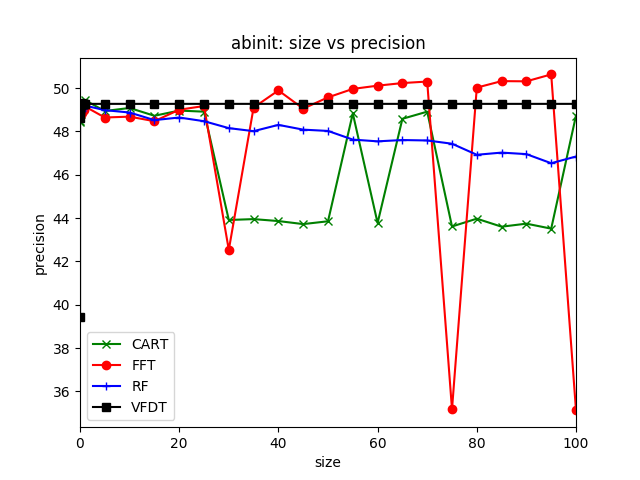
\includegraphics[width=6cm,height=4cm,keepaspectratio]{fig/abinit-size-precision.png}
	\caption{Size vs Precision for abinit dataset}
	\label{fig:ab-size-prec}
\end{figure}

\begin{figure}[h]
	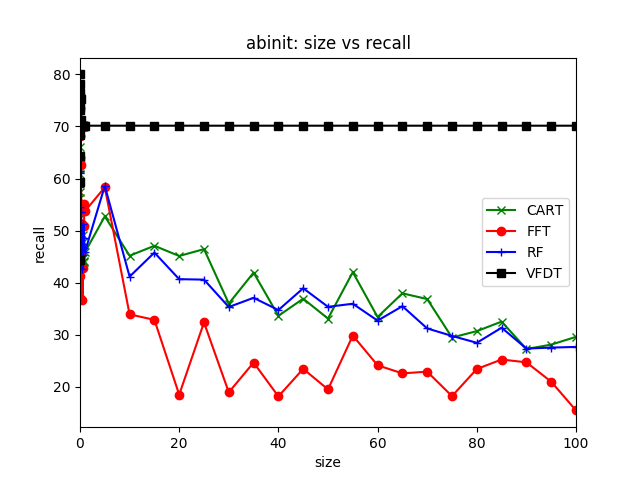
\includegraphics[width=6cm,height=4cm,keepaspectratio]{fig/abinit-size-recall.png}
	\caption{Size vs Recall for abinit dataset}
	\label{fig:ab-size-rec}
\end{figure}

From the figure \ref{fig:ab-size-prec} and \ref{fig:ab-size-prec} we can see that, with increase of the examples in abinit dataset, precision score for VFDT does not fluctuate but for the other three learners, it fluctuates, mostly FFT. However, in case of recall score, VFDT performs far better and stable across all of the sizes for the dataset. For the other three learners, the score gets lower and lower when the size increases. 

\begin{figure}[h]
	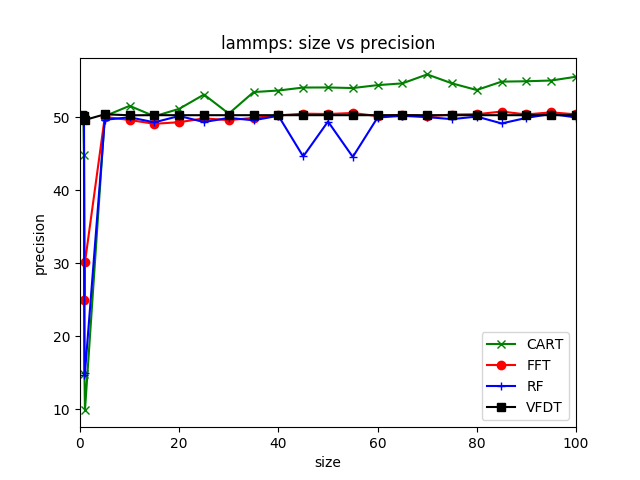
\includegraphics[width=6cm,height=4cm,keepaspectratio]{fig/lammps-size-precision.png}
	\caption{Size vs Precision for lammps dataset}
	\label{fig:lm-size-prec}
\end{figure}

\begin{figure}[h]
	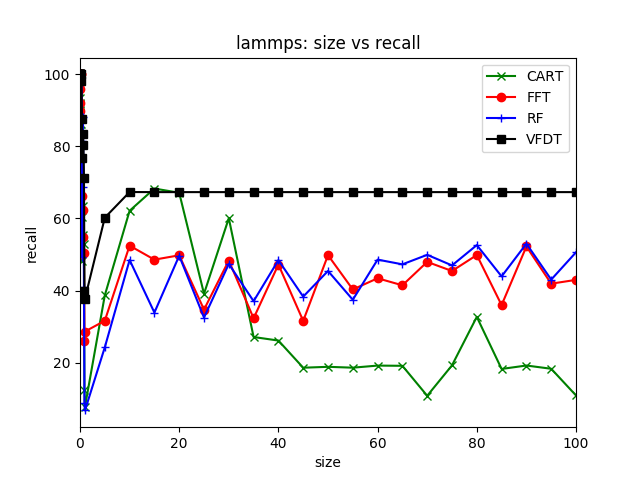
\includegraphics[width=6cm,height=4cm,keepaspectratio]{fig/lammps-size-recall.png}
	\caption{Size vs Recall for lammps dataset}
	\label{fig:lm-size-rec}
\end{figure}

From the figure \ref{fig:lm-size-prec} and \ref{fig:lm-size-prec} we can see that, with increase of the examples in lammps dataset, precision score for all the learners are similar and CART is performing slightly better than the others However, in case of recall score, VFDT slightly performs far better and stable across all of the sizes for the dataset. For the other three learners, the score fluctuates back and forth. However, CART performs the worst among the four learners. 

\begin{figure}[h]
	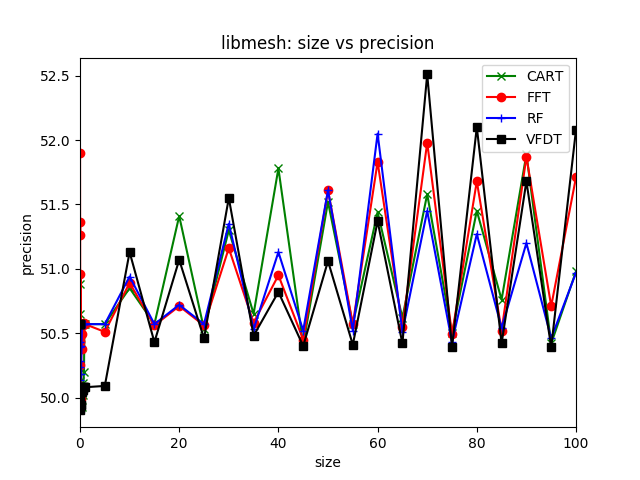
\includegraphics[width=6cm,height=4cm,keepaspectratio]{fig/libmesh-size-precision.png}
	\caption{Size vs Precision for libmesh dataset}
	\label{fig:lb-size-prec}
\end{figure}

\begin{figure}[h]
	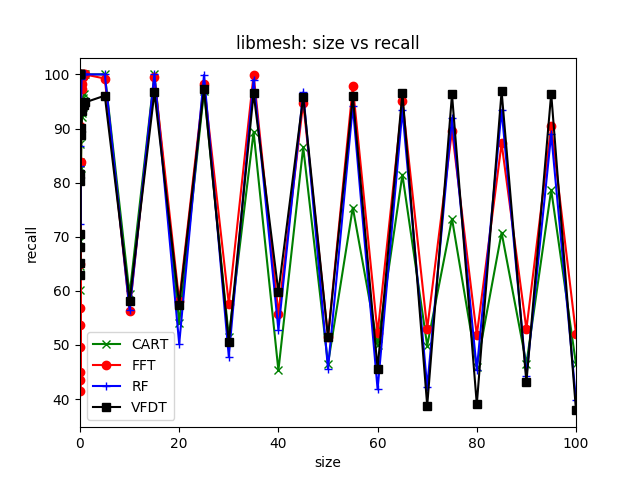
\includegraphics[width=6cm,height=4cm,keepaspectratio]{fig/libmesh-size-recall.png}
	\caption{Size vs Recall for libmesh dataset}
	\label{fig:lb-size-rec}
\end{figure}

From the figure \ref{fig:lb-size-prec} and \ref{fig:lb-size-prec} we can see that, with increase of the examples in libmesh dataset, precision and recall score for all the learners are similar. However, it also shows us that with the increase of dataset size, the recall scores behaves very unstable, for all of the four learners. 

\begin{figure}[h]
	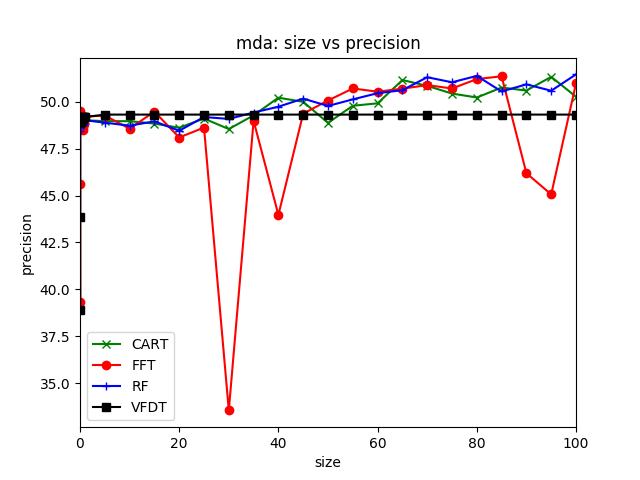
\includegraphics[width=6cm,height=4cm,keepaspectratio]{fig/mda-size-precision.png}
	\caption{Size vs Precision for mdanalysis dataset}
	\label{fig:md-size-prec}
\end{figure}

\begin{figure}[h]
	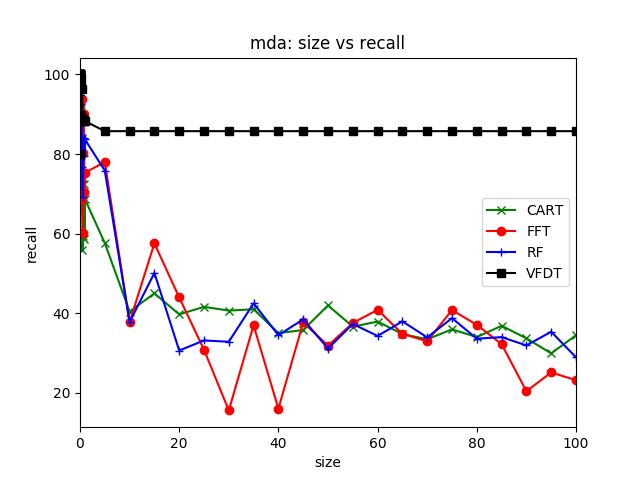
\includegraphics[width=6cm,height=4cm,keepaspectratio]{fig/mda-size-recall.png}
	\caption{Size vs Recall for mdanalysis dataset}
	\label{fig:md-size-rec}
\end{figure}

From the figure \ref{fig:md-size-prec} and \ref{fig:md-size-prec} we can see that, with increase of the examples in mdanalysis dataset, precision score for all the learners are similar and CART as well as FFT are performing slightly better than the others However, in case of recall score, VFDT performs far better and stable across all of the sizes for the dataset. For the other three learners, the score fluctuates back and forth a ittle bit. However, FFT performs the worst among the four learners. 

\begin{figure}[h]
	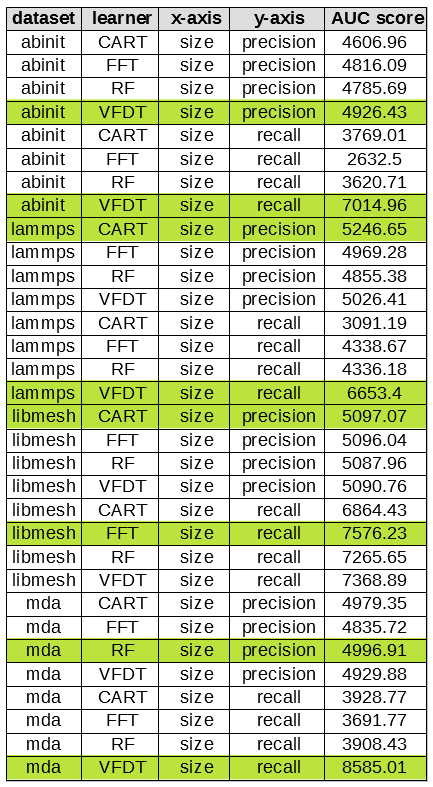
\includegraphics[width=\linewidth]{fig/auc-size.png}
	\caption{Size vs Recall for mdanalysis dataset}
	\label{fig:auc-size}
\end{figure}

..effort estimation

In principle, the key observation from the analysis of four datasets are given below: 
\begin{itemize}
	\item VFDT performs better in recall score across all the dataset size. This can also be seen in the AUC score given in \ref{fig:auc-size}
	\item VFDT achieves slightly a lower precision score than the other three learners. This can also be seen in the AUC score given in \ref{fig:auc-size}
	\item Precision and recall scores of all the three learners except VFDT either goes up or down with the increase of data fed into them. For VFDT, it remains stable. As, VFDT reaches hoeffding bound and grows tree accordingly, with the increase of the data size, it's tree structure does not change. Hence, its precision and recall score also stay unchanged.
	\item As we performed tuning of the learners with $25\%$ of the examples, it is obvious that optimal parameters for VFDT did not change while newer examples came. But with the arrival of newer examples, optimal set of parameters of CART and RF have changes. This is why their precision and recall score dropped.  
	\item the precision score also tells us that all the learner performed marginally better than a random guess. 
\end{itemize}

\subsection{RQ2: How hyper-parameters changes as the data size changes}
From the analysis in previous section, it is obvious that when the learner faces substantial amount of newer examples, their prediction performance goes down. Consequently, it remains to be seen whether further parameter tuning improves their performance or not. Keeping this in mind, we perform another three parameter tuning while the datasets finished processing $50\%$, $75\%$ and $100\%$ of the total examples. We observed that precision score does not vary significantly across the dataset size from all the learners, hence in our differential evolution method, we tried to optimize the parameters on the basis of recall score. Here is the summary of the findings:

\begin{figure}[h]
	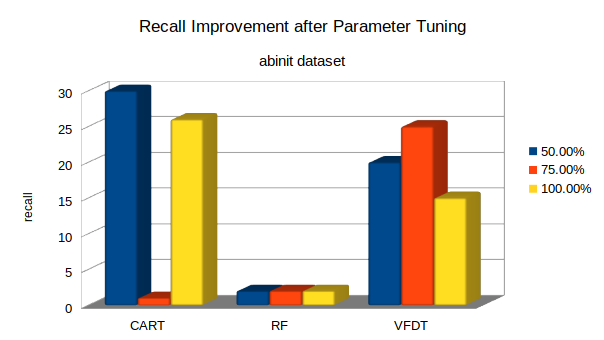
\includegraphics[width=\linewidth]{fig/tune-ab.png}
	\caption{Size vs Recall for mdanalysis dataset}
	\label{fig:tune-ab}
\end{figure}

\begin{figure}[h]
	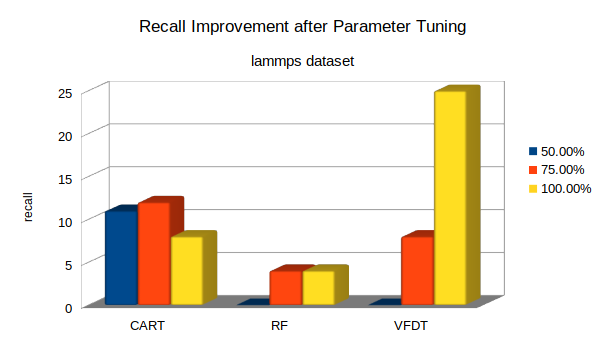
\includegraphics[width=\linewidth]{fig/tune-lm.png}
	\caption{Size vs Recall for mdanalysis dataset}
	\label{fig:tune-lm}
\end{figure}

\begin{figure}[h]
	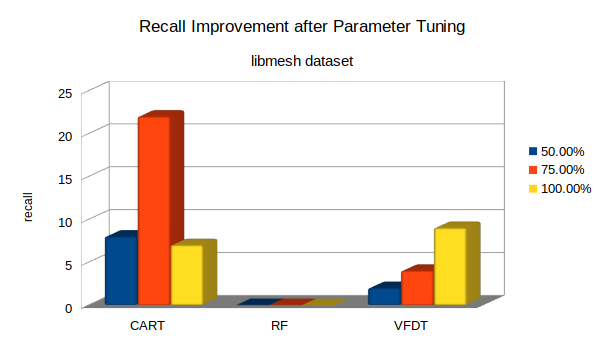
\includegraphics[width=\linewidth]{fig/tune-lb.png}
	\caption{Size vs Recall for mdanalysis dataset}
	\label{fig:tune-lb}
\end{figure}

\begin{figure}[h]
	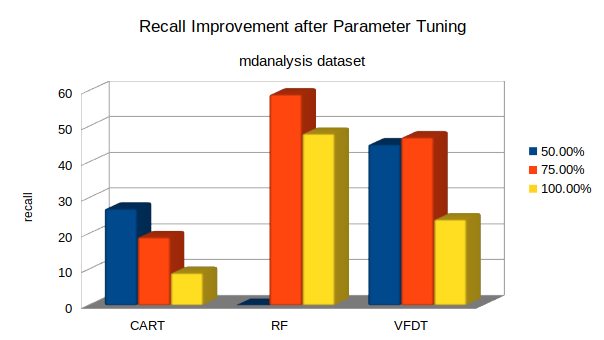
\includegraphics[width=\linewidth]{fig/tune-md.png}
	\caption{Size vs Recall for mdanalysis dataset}
	\label{fig:tune-md}
\end{figure}

It is obvious from Figure \ref{fig:tune-ab}, \ref{fig:tune-lm}, \ref{fig:tune-lb}, \ref{fig:tune-md} that, for most of the cases recall score could have been improved if further tuning was deployed after seeing a substantial amount of newer examples. However, in case of learning for a large stream of data periodically, it is really inefficient to apply tuning each time the dataset learns. 

\subsection{RQ3: How much computation resources would be used by these four learners}
It is also important to observe the computational resources being used by the learners because, with the increase of data size, the need for the learners to become cheap in terms of time and memory is paramount. Here, the findings from our analysis is presented below.

\begin{figure}
	\centering
	\begin{subfigure}[b]{\linewidth}
		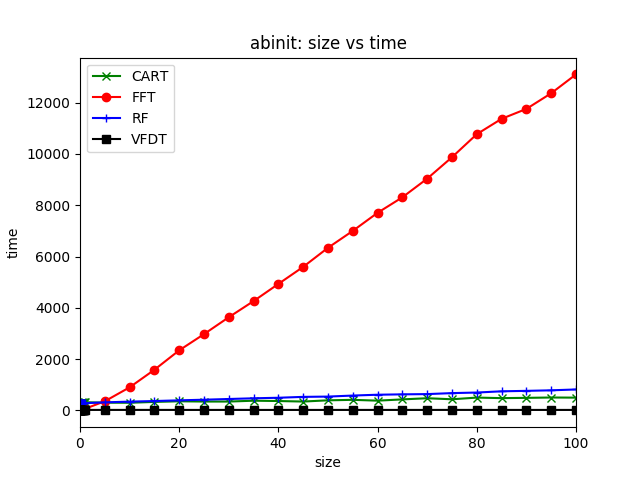
\includegraphics[width=.49\linewidth]{fig/abinit-size-time.png} \ 
		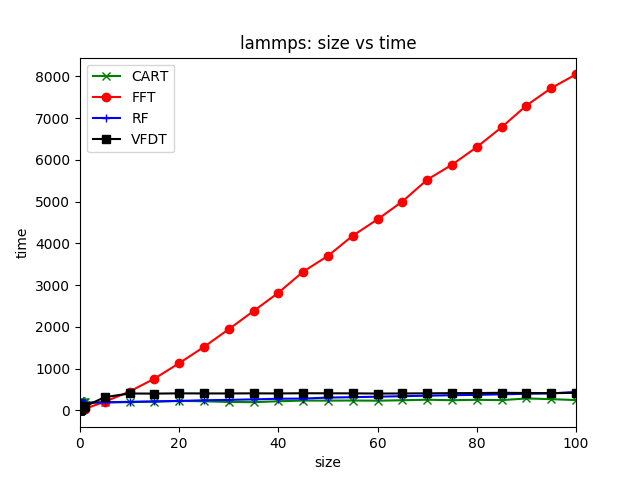
\includegraphics[width=.49\linewidth]{fig/lammps-size-time.png}
	\end{subfigure}
	\begin{subfigure}[b]{\linewidth}
		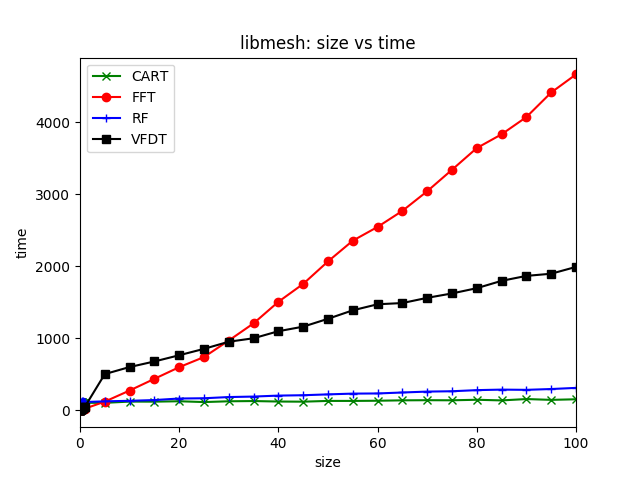
\includegraphics[width=.49\linewidth]{fig/libmesh-size-time.png} \ 
		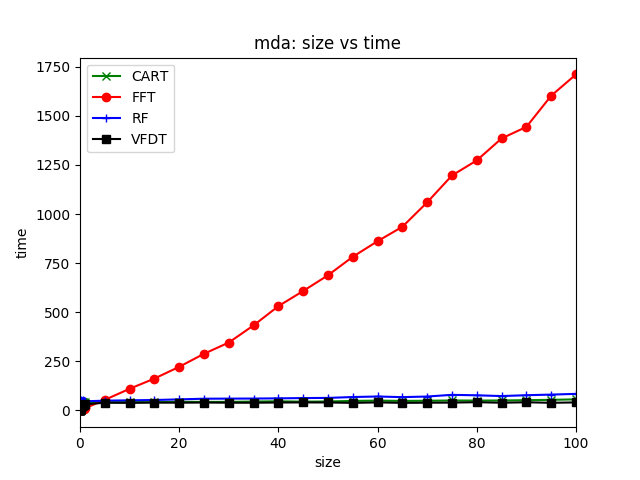
\includegraphics[width=.49\linewidth]{fig/mda-size-time.png}
	\end{subfigure}
	
	\caption{Data Size vs Time}\label{fig:time}
\end{figure}

From the above fig \ref{fig:time}, we can see that FFT is very expensive in terms of computation time. Apart from libmesh dataset, it is also seen that CART, RF and VFDT all takes similar time to operate. However, such comparison between VFDT, CART and RF is not conclusive as the dataset is very small compared to the available primary memory in the testbed system. Hence, we needed to deploy the learner with a very big dataset that is similar to the size of primary memory of the computer. Unfortunately, such big dataset is not available for software defect prediction. Hence, we collected particle acceleration dataset from UCI Machine Learning dataset repository. The size of the dataset is around $8$Gb of size. It contains $110000000$ rows and $29$ columns. All the class labels are either boolean and attributes are continuous. From our run, here is the outcome. From the table \ref{higgs} above, it is obvious that VFDT scales in terms of both computation time and memory usage if the dataset size is substantially large.

\begin{table}
	\begin{tabular}{|c|c|c|}
		\hline 
		\textbf{Learner} & \textbf{Time} & Me\textbf{}mory \\ 
		\hline 
		CART & 654k & 14GB \\ 
		\hline 
		RF & 895k & 14Gb \\ 
		\hline 
		VFDT & 5.2k & 1.2GB \\ 
		\hline 
	\end{tabular}
	\caption{Computation Resource Usage for Very Large Dataset} 
	\label{higgs}
\end{table}

\section{Threats to Validity}



%\section{Threats to Validity}

%\section{Future Work Direction and Conclusion}

%% Bibliography
\bibliography{bibfile}
\bibliographystyle{ACM-Reference-Format}
%
%
%%% Appendix
%\appendix
%\section{Appendix}


\end{document}
